\begin{figure}[!ht]
    \centering 
    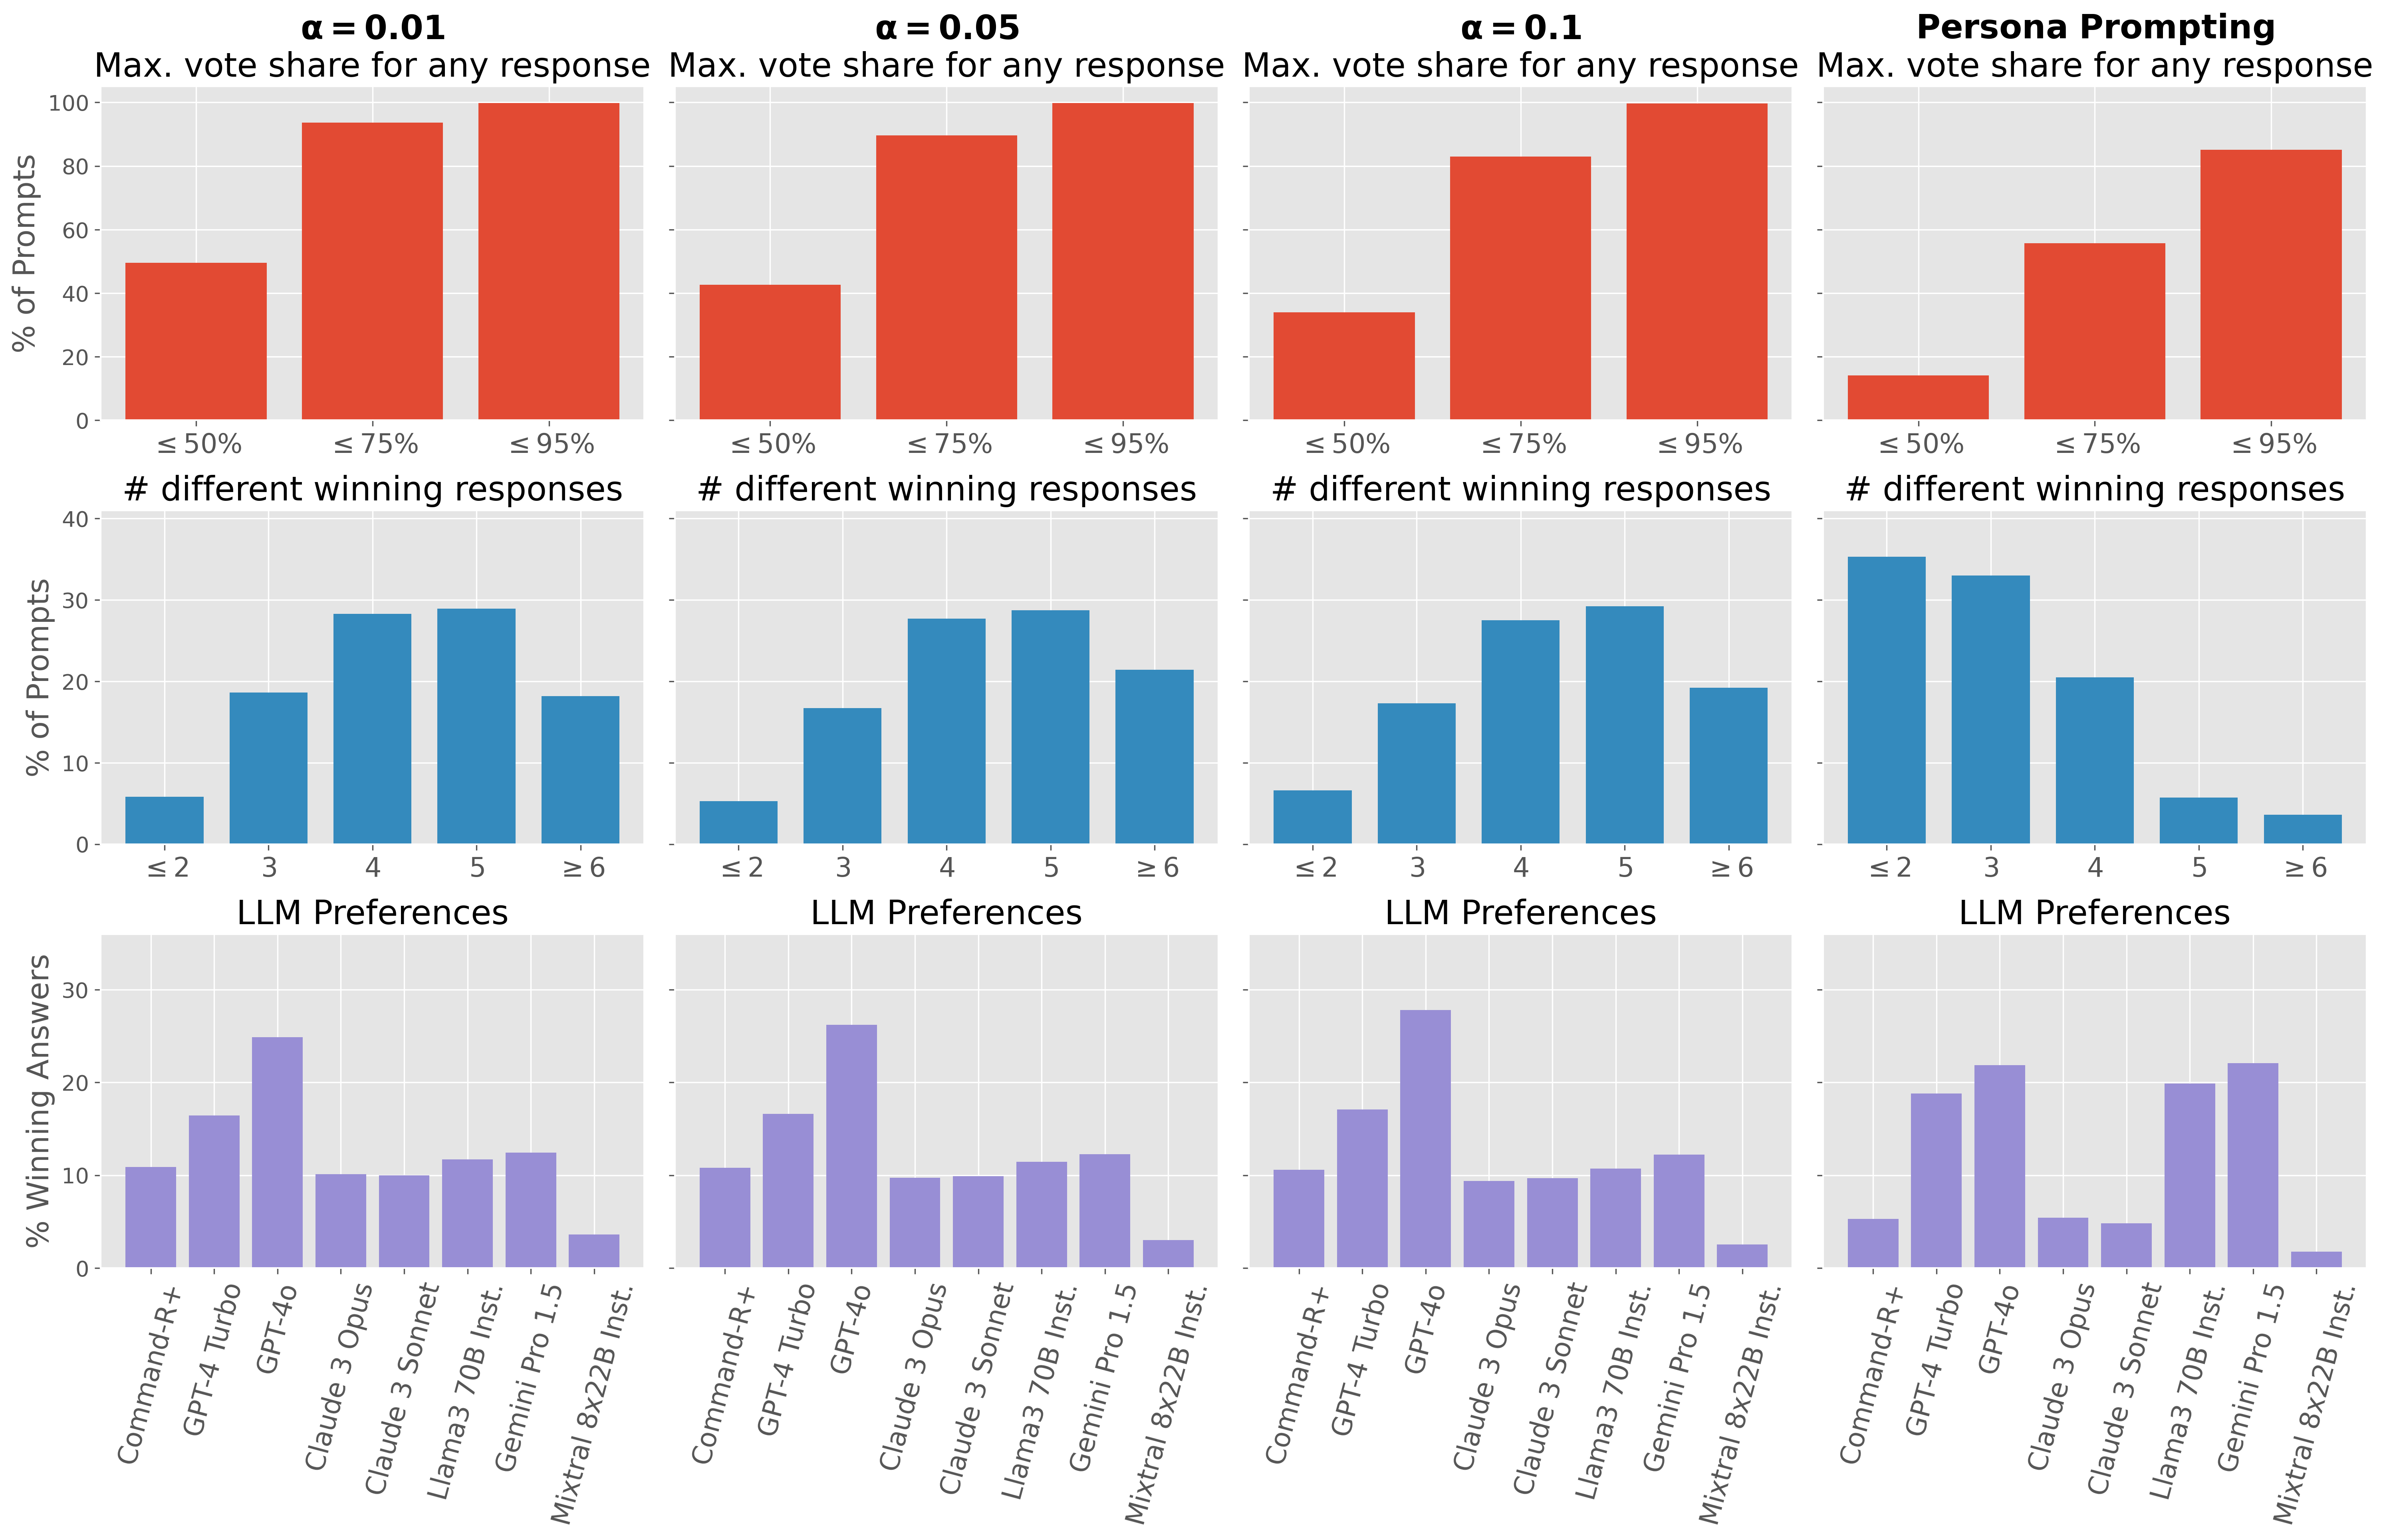
\includegraphics[width=\linewidth]{figures/persona_prompting_comparison.png}
    \caption{Probing the heterogeneous preferences across \textsf{PersonalLLM} prompt/responses given different settings of $\alpha$, and comparing to a persona prompting baseline.  \textbf{Top}: For a population of simulated users, the percentage of each population's vote share given to the most common winning response for each prompt; higher values indicate more preference diversity. \textbf{Middle}: A histogram showing the number of responses that receive at least one vote from a simulated population for each prompt; diverse preferences cause higher concentration on the right side of each plot. \textbf{Bottom}: Average win rates across the population for the 8 LLMs in our dataset.}
    \label{fig:persona_diversity}
\end{figure}

\section{Analyzing PersonalLLM}\label{sec:persona_analysis}

Next, in order to validate our testbed, we explore the preferences exhibited by our simulated users over the \textsf{PersonalLLM} dataset.  

\subsection{Preference Diversity and Comparison to Persona Prompting}
% \hntodo{Enlarge figure titles, axis labels A LOT! Rule of thumb is whether it's clearly legible if printed on a letter sized paper. Figure 4 is especially challenging to read since the x-axis is different across rows. In the caption, it may be worth explicitly saying higher proportions on the left hand side implies greater diversity or something like this to help people skim the figure.}

First, we examine whether populations of personal preference models sampled via the method outlined in Section~\ref{sec:sim_users} do in fact display heterogeneous preferences over the prompt/response pair in our dataset.
In Figure~\ref{fig:persona_diversity} (left 3 columns), we provide experimental results for user bases of 1,000 \textsf{PersonalLLM} personal preference models sampled with parameters $\alpha=[0.01, 0.05, 0.1]$ and applied to the \textsf{PersonalLLM} test set to choose winning responses among the 8 included.
The top row displays the percentage of prompts in the dataset for which the most popular winning response according to the population receives no more than 50\%, 75\%, and 95\% of the population vote; higher values indicate more diversity in preferred responses.  
The middle row shows the percentage of prompts that have a given number of responses with at least one winning vote across the population; heterogeneous population preferences induce higher concentration on the right side of each plot.
On the bottom, we plot the overall win rates for each LLM across all users and prompts.

In the right column, we also offer results for a persona prompting baseline.  
Persona prompting \citep{castricato2024personareproducibletestbedpluralistic, chan2024scalingsyntheticdatacreation, jang2023personalizedsoupspersonalizedlarge} is an emerging method for evaluating methods for LLM personalization, wherein an LLM is prompted to decide which response would be preferred by a person of a particular race, gender, age, profession, or other demographic category.  
While one might argue that such evaluation is \textit{prima facie} discriminatory and reductive, and therefore not a desirable standard for algorithmic advancement, especially in sensitive areas, we are also interested in whether persona prompting meets the technical challenge of producing a simulation environment with a high degree of heterogeneity.
For our baseline, we prompt the sfairXC/FsfairX-LLaMA3-RM-v0.1 reward model \citep{dong2023raft} to score responses with respect to 500 personas randomly sampled from PersonaHub \citet{chan2024scalingsyntheticdatacreation}, a recent effort at building a database of personas that are representative of a pluralistic population.

Results are shown in Figure~\ref{fig:persona_diversity}.
For \textsf{PersonalLLM} personas, we can see that the top response receives a majority user vote for only about half of the prompts, while that figure is closer to 90\% for the persona prompting baseline.  
Also, for roughly 60\% of prompts, at least 5 different answers are chosen as the best by at least 1 under our set of personas; for LLM persona prompting, it is roughly 30\%.  
Finally, our ensembled preference models have a fairly diffuse set of preferences over the response-generating LLMs, while persona prompting strongly prefers a subset of 4 models.
With respect to changes across the left 3 columns, we can observe that as $\alpha$ increases, preferences become more uniform.  
However, if $\alpha$ is set too low, user preferences cluster very tightly around the base reward models; we observe this behavior for $\alpha=0.01$.

\begin{figure}[t]
    \centering 
    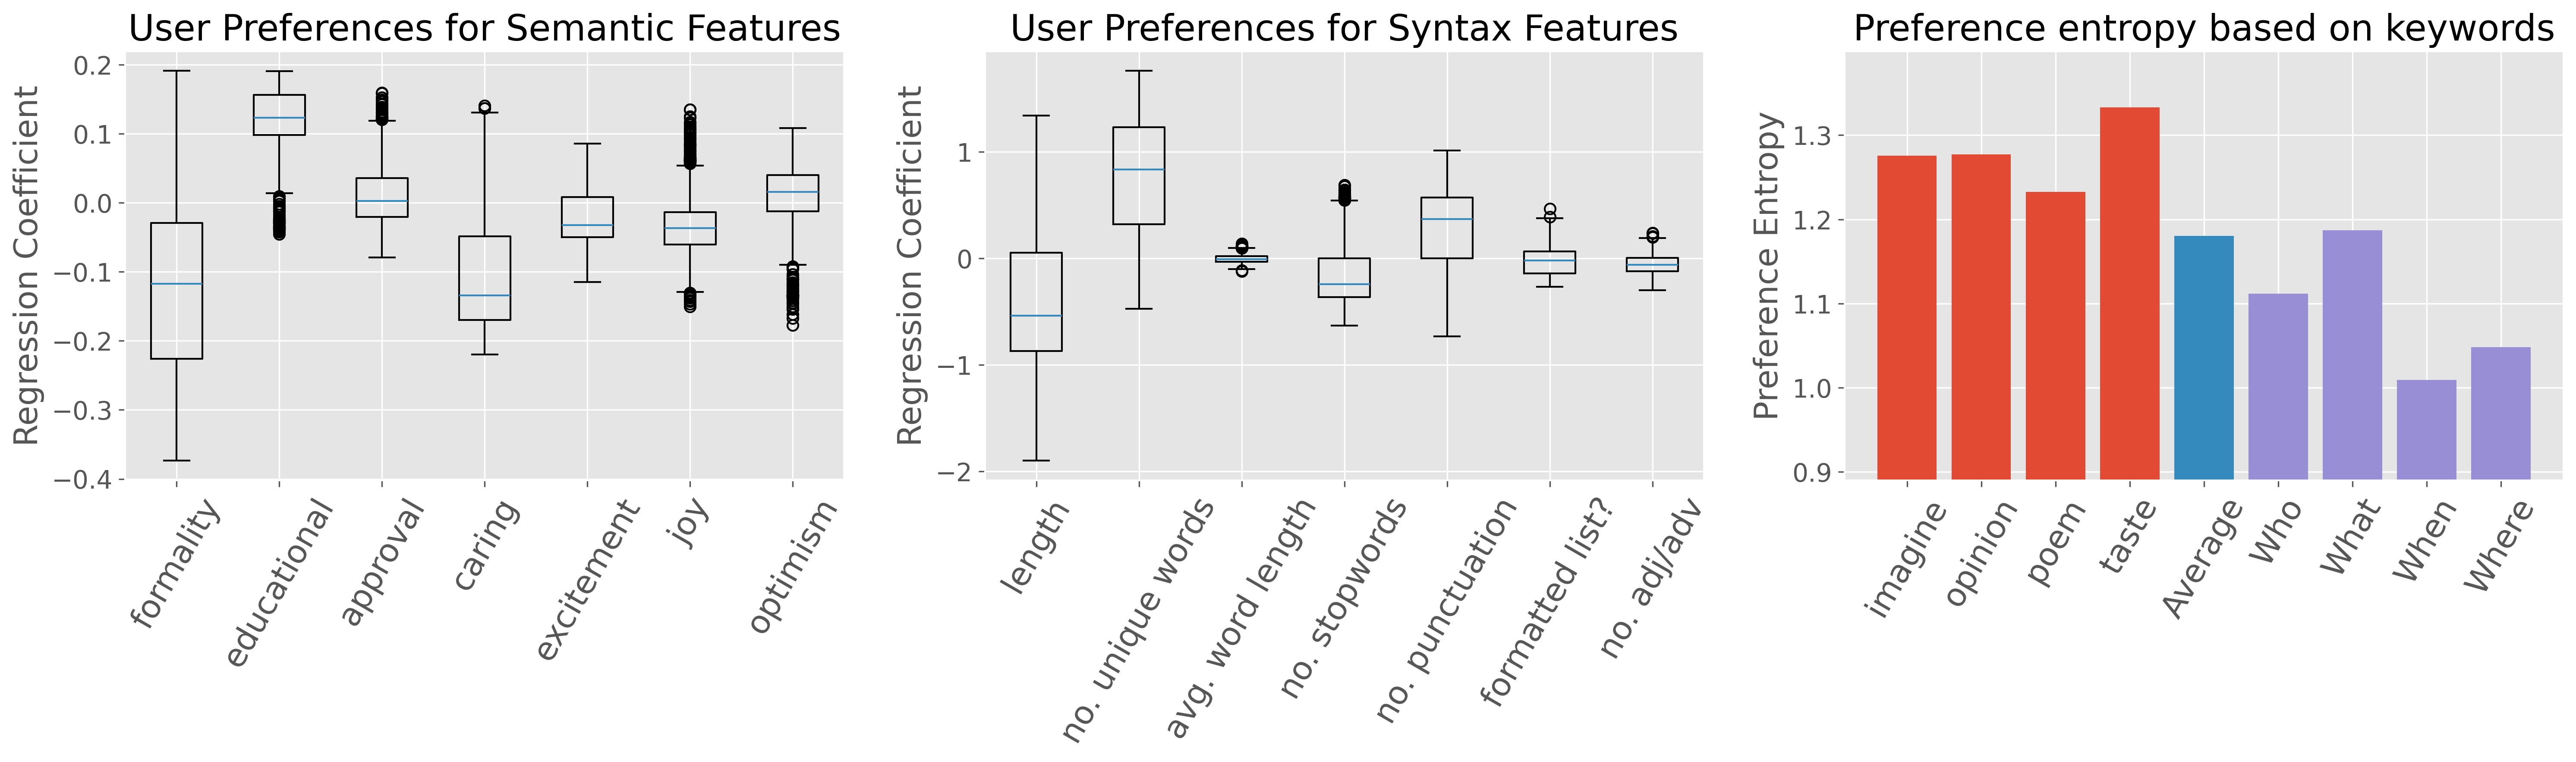
\includegraphics[width=\linewidth]{figures/syn_sem_ent.png}
    \caption{Analysis of simulated user preferences with respect to prompt and response contents.
    \textbf{Left, middle:} For each user, we train a regression model to predict winning responses based on either semantic (left) or syntactic (middle) features.  For each feature, we show a box plot with the resultant regression coefficient across users.
    \textbf{Right:} We examine the entropy in population preferences based on keywords in prompts, comparing words we would expect to inspire heterogeneity (e.g., imagine, opinion, poem) to prompts beginning with who, when, and where, which should evoke more objective answers. 
    }
    \label{fig:sem_syn}
\end{figure}

\subsection{Effects of Semantics and Syntax}

% \hntodo{Enlarge figure titles, axis labels A LOT! Rule of thumb is whether it's clearly legible if printed on a letter sized paper}

We further analyze the effects of semantics and syntax on the preferences of a simulated user base (with $\alpha=0.05$ and 1,000 users).  We use regression analysis to understand how different features may drive the preferences of different users, including semantic response features such as the formality or educational value or the expressions of certain emotions (approval, caring, excitement, joy, optimism), as well as syntactic features like length and the use of different parts of speech and formatting.
For each user, we gather their most and least preferred responses for each of the test prompts, and create a binary prediction problem to predict whether a given response is a winning or losing response.
Responses are embedded using hand-crafted features (based on either syntax or semantics, which are studied separately), and a unique logistic regression model is trained \textit{for each user}.
Semantic features were captured using pretrained classifiers, while syntactic features were engineered using nltk \citep{bird-loper-2004-nltk}.  See Appendix \ref{app:user_details} for complete details.

In Figure~\ref{fig:sem_syn} (left and middle), for each feature we show a box plot with the resultant regression coefficient for that feature across users.  A positive coefficient suggests a feature associated with winning responses, while a negative coefficient suggests a feature's role in losing responses.  A tight box indicates homogeneous preferences, while a greater spread represents heterogeneity.
Here, we can see a reasonable mix of heterogeneity and homogeneity across user preferences for different features. 
Semantically, users tend to prefer responses with educational value and dislike highly formal responses, although the size of these preferences varies.
Encouragingly, syntactic preferences do not seem to be driven by uniform preferences for simple features like length or the presence of formatting such as bullets or lists.

In Figure~\ref{fig:sem_syn} (right), we compare the entropy in the population preferences over the responses to a given prompt based on keywords, comparing words we would expect to inspire heterogeneity (e.g., imagine, opinion, poem) to prompts beginning with who, when, and where, which evoke more objective answers.  We can see that the presence of these subjective cues leads to a more diverse set of preferences than those seeking simple entity or date responses.  Such diversity among the prompts creates a setting where an algorithm \textit{must not only learn how to personalize, but also when to personalize}.
% \hntodo{Consider moving much of the figure descriptions to the caption. Currently readers will need to read the subsection carefully to comprehend the plots. Most will start with the initial paragraph and then move to the figure to stare at them.}

\subsection{Comparison to Human Preferences}

% \hntodo{Perhaps give a couple of real examples from OpinionQA to ground our analysis.}
Finally, to understand how our synthetic personal preference models relate to human preferences over text responses, we surveyed a population of our simulated users on a set of questions with responses where a large and diverse set of humans have given their preferences in the past, the OpinionQA dataset
% , emulating the work of 
\citep{santurkar2023opinions}.
OpinionQA is an appropriate validation set for our personas given that its broad coverage of topics (e.g., science, economics, politics, romance, and many other topics) aligns with the open-domain nature of our prompt set.  See Table~\ref{tab:opinion_qa_examples} for example questions and answers.

\begin{table}[!ht]
    \centering
    \begin{tabular}{p{0.55\textwidth} p{0.4\textwidth}}
    \toprule
     Question & Answer\\
    \midrule
    How worried are you, if at all, about the possibility of using computer programs to make hiring decisions for society as a whole? & [Very worried, Somewhat worried, Not too worried, Not at all worried] \\
    \midrule
    Do you think men and women are basically similar or basically different when it comes to their hobbies and personal interests? & [Men and women are basically similar, Men and women are basically different] \\
    \bottomrule
    \end{tabular}
    \caption{Example questions and answers from the OpinionQA dataset.}
    \label{tab:opinion_qa_examples}

\end{table}

Following this previous work, we calculate the representativeness score of the opinion distribution given by our simulated preference models.
This score is based on the Wasserstein distance of the synthetic population preferences from that of real human populations for each question.
To have a high representativeness score, our simulated user population would have to display heterogeneous preferences over question/response sets where humans do so, and produce homogeneous (and matching) preferences in cases where humans do the same. 

Our population of simulated users produces a representativeness score of 0.839 with respect to the overall population of the US, higher than any LLM in the original study and near as representative of the overall population as some real, large demographic groups.  
Further, in Table~\ref{tab:opinion_qa} we can see that our simulated users produce opinions that better represent a wide range of important (and sometimes protected) groups according to demographic attributes such as race, political leaning, religion, marital status, and more.  
In fact, this is the case for 59 of 60 demographic groups in their study (see Appendix Table~\ref{tab:opinion_qa_full}).

\begin{table}[!ht]
    \centering
    \begin{tabular}{lccccc}
    \toprule
     & \multicolumn{2}{c}{AI21 Labs} & \multicolumn{2}{c}{OpenAI} & \textsf{PersonalLLM} \\
    Demographic & j1-jumbo & j1-grande-v2 & ada & text-davinci-003 & \textbf{Ours} \\
    \midrule
    Asian & 0.814 & 0.806 & 0.819 & 0.708 & \textbf{0.839} \\
    Black & 0.820 & 0.812 & 0.823 & 0.702 & \textbf{0.833} \\
    Hispanic & 0.820 & 0.810 & 0.824 & 0.706 & \textbf{0.839} \\
    White & 0.807 & 0.794 & 0.817 & 0.699 & \textbf{0.832} \\
    Conservative & 0.796 & 0.780 & 0.810 & 0.684 & \textbf{0.817} \\
    Liberal & 0.792 & 0.788 & 0.799 & 0.721 & \textbf{0.833} \\
    Democrat & 0.800 & 0.795 & 0.804 & 0.719 & \textbf{0.834} \\
    Republican & 0.791 & 0.776 & 0.805 & 0.680 & \textbf{0.812} \\
    Muslim & 0.794 & 0.788 & 0.792 & 0.697 & \textbf{0.816} \\
    Roman Catholic & 0.816 & 0.806 & 0.823 & 0.702 & \textbf{0.835} \\
    Less than \$30,000 & 0.828 & 0.813 & 0.833 & 0.693 & \textbf{0.838} \\
    \$100,000 or more & 0.797 & 0.790 & 0.807 & 0.708 & \textbf{0.831} \\
    18-29 & 0.818 & 0.808 & 0.828 & 0.700 & \textbf{0.840} \\
    65+ & 0.792 & 0.779 & 0.800 & 0.699 & \textbf{0.818} \\
    Divorced & 0.809 & 0.796 & 0.817 & 0.696 & \textbf{0.830} \\
    Married & 0.810 & 0.799 & 0.819 & 0.699 & \textbf{0.832} \\
    \bottomrule
    \end{tabular}
    \caption{Representativeness scores in relation to real human opinions from important demographic groups for different LLMs, as well as our \textsf{PersonalLLM} population.}
    \label{tab:opinion_qa}
\end{table}

\subsection{Summary of Analysis}

Taken together, these results show that our simulated user reward models: 1) produce heterogeneous preferences over our dataset of prompts and responses, considerably more so than persona prompting an LLM, 2) display reasonable and diverse preferences with respect to syntactic and semantic content of prompts, and 3) simulate a user base that better represents diverse human opinions than many popular LLMs, without resorting to explicit stereotyping.
% \hntodo{Claiming better representation of real human opinions may be untenable. One option is to focus on diversity and heterogeneity rather than realism.}


